\chapter{Análisis amortizado}

\index{análisis amortizado}

La complejidad temporal de un algoritmo
a menudo es fácil de analizar
simplemente examinando la estructura
del algoritmo:
qué bucles contiene el algoritmo
y cuántas veces se realizan los bucles.
Sin embargo, a veces un análisis directo
no proporciona una imagen real de la eficiencia del algoritmo.

El \key{Análisis amortizado} se puede utilizar para analizar
algoritmos que contienen operaciones cuya
complejidad temporal varía.
La idea es estimar el tiempo total utilizado en
todas estas operaciones durante la
ejecución del algoritmo, en lugar de centrarse
en operaciones individuales.

\section{Método de dos punteros}

\index{método de dos punteros}

En el \key{método de dos punteros},
se utilizan dos punteros para
iterar a través de los valores del arreglo.
Ambos punteros pueden moverse en una dirección solamente,
lo que garantiza que el algoritmo funcione de manera eficiente.
A continuación, discutimos dos problemas que se pueden resolver
utilizando el método de dos punteros.

\subsubsection{Suma de subarreglo}

Como primer ejemplo,
consideremos un problema en el que se nos da
un arreglo de $n$ enteros positivos
y una suma objetivo $x$,
y queremos encontrar un subarreglo cuya suma sea $x$
o informar que no existe tal subarreglo.

Por ejemplo, el arreglo
\begin{center}
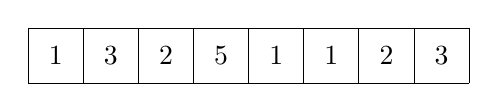
\begin{tikzpicture}[scale=0.7]
\draw (0,0) grid (8,1);

\node at (0.5,0.5) {$1$};
\node at (1.5,0.5) {$3$};
\node at (2.5,0.5) {$2$};
\node at (3.5,0.5) {$5$};
\node at (4.5,0.5) {$1$};
\node at (5.5,0.5) {$1$};
\node at (6.5,0.5) {$2$};
\node at (7.5,0.5) {$3$};
\end{tikzpicture}
\end{center}
contiene un subarreglo cuya suma es 8:
\begin{center}
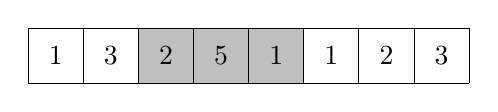
\begin{tikzpicture}[scale=0.7]
\fill[color=lightgray] (2,0) rectangle (5,1);
\draw (0,0) grid (8,1);

\node at (0.5,0.5) {$1$};
\node at (1.5,0.5) {$3$};
\node at (2.5,0.5) {$2$};
\node at (3.5,0.5) {$5$};
\node at (4.5,0.5) {$1$};
\node at (5.5,0.5) {$1$};
\node at (6.5,0.5) {$2$};
\node at (7.5,0.5) {$3$};
\end{tikzpicture}
\end{center}

Este problema se puede resolver en
$O(n)$ tiempo utilizando el método de dos punteros.
La idea es mantener punteros que apuntan al
primer y último valor de un subarreglo.
En cada turno, el puntero izquierdo se mueve un paso
a la derecha, y el puntero derecho se mueve a la derecha
siempre que la suma del subarreglo resultante sea como máximo $x$.
Si la suma se convierte exactamente en $x$,
se ha encontrado una solución.

Por ejemplo, considere el siguiente arreglo
y una suma objetivo $x=8$:
\begin{center}
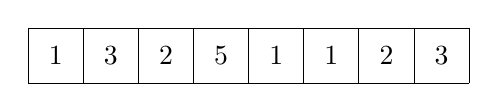
\begin{tikzpicture}[scale=0.7]
\draw (0,0) grid (8,1);

\node at (0.5,0.5) {$1$};
\node at (1.5,0.5) {$3$};
\node at (2.5,0.5) {$2$};
\node at (3.5,0.5) {$5$};
\node at (4.5,0.5) {$1$};
\node at (5.5,0.5) {$1$};
\node at (6.5,0.5) {$2$};
\node at (7.5,0.5) {$3$};
\end{tikzpicture}
\end{center}

El subarreglo inicial contiene los valores
1, 3 y 2 cuya suma es 6:

\begin{center}
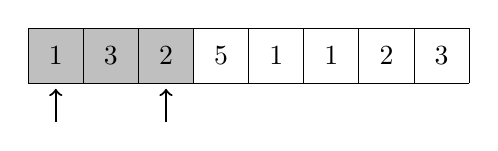
\begin{tikzpicture}[scale=0.7]
\fill[color=lightgray] (0,0) rectangle (3,1);
\draw (0,0) grid (8,1);

\node at (0.5,0.5) {$1$};
\node at (1.5,0.5) {$3$};
\node at (2.5,0.5) {$2$};
\node at (3.5,0.5) {$5$};
\node at (4.5,0.5) {$1$};
\node at (5.5,0.5) {$1$};
\node at (6.5,0.5) {$2$};
\node at (7.5,0.5) {$3$};

\draw[thick,->] (0.5,-0.7) -- (0.5,-0.1);
\draw[thick,->] (2.5,-0.7) -- (2.5,-0.1);
\end{tikzpicture}
\end{center}

Luego, el puntero izquierdo se mueve un paso a la derecha.
El puntero derecho no se mueve, porque de lo contrario
la suma del subarreglo excedería $x$.

\begin{center}
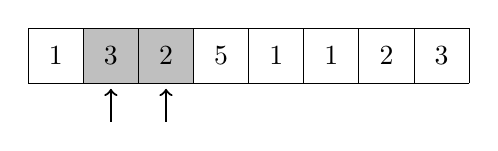
\begin{tikzpicture}[scale=0.7]
\fill[color=lightgray] (1,0) rectangle (3,1);
\draw (0,0) grid (8,1);

\node at (0.5,0.5) {$1$};
\node at (1.5,0.5) {$3$};
\node at (2.5,0.5) {$2$};
\node at (3.5,0.5) {$5$};
\node at (4.5,0.5) {$1$};
\node at (5.5,0.5) {$1$};
\node at (6.5,0.5) {$2$};
\node at (7.5,0.5) {$3$};

\draw[thick,->] (1.5,-0.7) -- (1.5,-0.1);
\draw[thick,->] (2.5,-0.7) -- (2.5,-0.1);
\end{tikzpicture}
\end{center}

De nuevo, el puntero izquierdo se mueve un paso a la derecha,
y esta vez el puntero derecho se mueve tres
pasos a la derecha.
La suma del subarreglo es $2+5+1=8$, entonces se ha encontrado un subarreglo
cuya suma es $x$.

\begin{center}
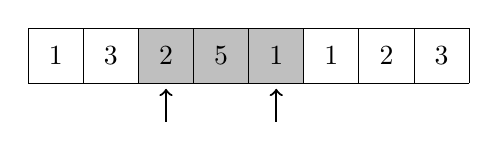
\begin{tikzpicture}[scale=0.7]
\fill[color=lightgray] (2,0) rectangle (5,1);
\draw (0,0) grid (8,1);

\node at (0.5,0.5) {$1$};
\node at (1.5,0.5) {$3$};
\node at (2.5,0.5) {$2$};
\node at (3.5,0.5) {$5$};
\node at (4.5,0.5) {$1$};
\node at (5.5,0.5) {$1$};
\node at (6.5,0.5) {$2$};
\node at (7.5,0.5) {$3$};

\draw[thick,->] (2.5,-0.7) -- (2.5,-0.1);
\draw[thick,->] (4.5,-0.7) -- (4.5,-0.1);
\end{tikzpicture}
\end{center}

El tiempo de ejecución del algoritmo depende de
la cantidad de pasos que el puntero derecho se mueva.
Si bien no hay un límite superior útil sobre cuántos pasos puede
moverse el puntero en un \emph{único} turno,
sabemos que el puntero se mueve \emph{un total de}
$O(n)$ pasos durante el algoritmo,
porque solo se mueve hacia la derecha.

Dado que tanto el puntero izquierdo como el derecho
se mueven $O(n)$ pasos durante el algoritmo,
el algoritmo funciona en tiempo $O(n)$.

\subsubsection{Problema 2SUM}

\index{Problema 2SUM}

Otro problema que se puede resolver usando
el método de dos punteros es el siguiente problema,
también conocido como el problema \key{2SUM}:
dado un arreglo de $n$ números y
una suma objetivo $x$, encuentre
dos valores del arreglo tales que su suma sea $x$,
o informe que no existen tales valores.

Para resolver el problema, primero
ordenamos los valores del arreglo en orden creciente.
Después de eso, iteramos a través del arreglo usando
dos punteros.
El puntero izquierdo comienza en el primer valor
y se mueve un paso a la derecha en cada turno.
El puntero derecho comienza en el último valor
y siempre se mueve hacia la izquierda hasta que la suma de los
valores izquierdo y derecho sea como máximo $x$.
Si la suma es exactamente $x$,
se ha encontrado una solución.

Por ejemplo, considere el siguiente arreglo
y una suma objetivo $x=12$:
\begin{center}
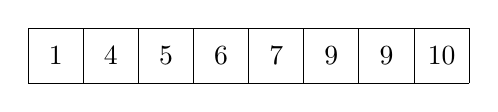
\begin{tikzpicture}[scale=0.7]
\draw (0,0) grid (8,1);

\node at (0.5,0.5) {$1$};
\node at (1.5,0.5) {$4$};
\node at (2.5,0.5) {$5$};
\node at (3.5,0.5) {$6$};
\node at (4.5,0.5) {$7$};
\node at (5.5,0.5) {$9$};
\node at (6.5,0.5) {$9$};
\node at (7.5,0.5) {$10$};
\end{tikzpicture}
\end{center}

Las posiciones iniciales de los punteros
son las siguientes.
La suma de los valores es $1+10=11$
que es menor que $x$.

\begin{center}
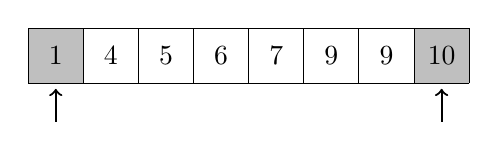
\begin{tikzpicture}[scale=0.7]
\fill[color=lightgray] (0,0) rectangle (1,1);
\fill[color=lightgray] (7,0) rectangle (8,1);
\draw (0,0) grid (8,1);

\node at (0.5,0.5) {$1$};
\node at (1.5,0.5) {$4$};
\node at (2.5,0.5) {$5$};
\node at (3.5,0.5) {$6$};
\node at (4.5,0.5) {$7$};
\node at (5.5,0.5) {$9$};
\node at (6.5,0.5) {$9$};
\node at (7.5,0.5) {$10$};

\draw[thick,->] (0.5,-0.7) -- (0.5,-0.1);
\draw[thick,->] (7.5,-0.7) -- (7.5,-0.1);
\end{tikzpicture}
\end{center}

Luego, el puntero izquierdo se mueve un paso a la derecha.
El puntero derecho se mueve tres pasos a la izquierda,
y la suma se convierte en $4+7=11$.

\begin{center}
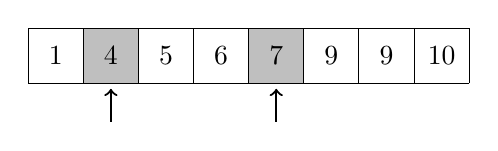
\begin{tikzpicture}[scale=0.7]
\fill[color=lightgray] (1,0) rectangle (2,1);
\fill[color=lightgray] (4,0) rectangle (5,1);
\draw (0,0) grid (8,1);

\node at (0.5,0.5) {$1$};
\node at (1.5,0.5) {$4$};
\node at (2.5,0.5) {$5$};
\node at (3.5,0.5) {$6$};
\node at (4.5,0.5) {$7$};
\node at (5.5,0.5) {$9$};
\node at (6.5,0.5) {$9$};
\node at (7.5,0.5) {$10$};

\draw[thick,->] (1.5,-0.7) -- (1.5,-0.1);
\draw[thick,->] (4.5,-0.7) -- (4.5,-0.1);
\end{tikzpicture}
\end{center}

Después de esto, el puntero izquierdo se mueve un paso a la derecha nuevamente.
El puntero derecho no se mueve y se encuentra una solución
$5+7=12$.

\begin{center}
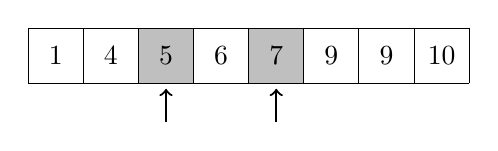
\begin{tikzpicture}[scale=0.7]
\fill[color=lightgray] (2,0) rectangle (3,1);
\fill[color=lightgray] (4,0) rectangle (5,1);
\draw (0,0) grid (8,1);

\node at (0.5,0.5) {$1$};
\node at (1.5,0.5) {$4$};
\node at (2.5,0.5) {$5$};
\node at (3.5,0.5) {$6$};
\node at (4.5,0.5) {$7$};
\node at (5.5,0.5) {$9$};
\node at (6.5,0.5) {$9$};
\node at (7.5,0.5) {$10$};

\draw[thick,->] (2.5,-0.7) -- (2.5,-0.1);
\draw[thick,->] (4.5,-0.7) -- (4.5,-0.1);
\end{tikzpicture}
\end{center}

El tiempo de ejecución del algoritmo es
$O(n \log n)$, porque primero ordena
el arreglo en tiempo $O(n \log n)$,
y luego ambos punteros se mueven $O(n)$ pasos.

Tenga en cuenta que es posible resolver el problema
de otra manera en tiempo $O(n \log n)$ usando búsqueda binaria.
En tal solución, iteramos a través del arreglo
y para cada valor del arreglo, intentamos encontrar otro
valor que produzca la suma $x$.
Esto se puede hacer realizando $n$ búsquedas binarias,
cada una de las cuales toma tiempo $O(\log n)$.

\index{problema 3SUM}
Un problema más difícil es
el \key{problema 3SUM} que pregunta por
encontrar \emph{tres} valores del arreglo
cuya suma sea $x$.
Usando la idea del algoritmo anterior,
este problema se puede resolver en tiempo $O(n^2)$\footnote{Durante mucho tiempo,
se pensó que resolver
el problema 3SUM de manera más eficiente que en tiempo $O(n^2)$
no sería posible.
Sin embargo, en 2014, resultó \cite{gro14}
que este no es el caso.}.
¿Puedes ver cómo?

\section{Nearest smaller elements}

\index{nearest smaller elements}

Amortized analysis is often used to
estimate the number of operations
performed on a data structure.
The operations may be distributed unevenly so
that most operations occur during a
certain phase of the algorithm, but the total
number of the operations is limited.

As an example, consider the problem
of finding for each array element
the \key{nearest smaller element}, i.e.,
the first smaller element that precedes the element
in the array.
It is possible that no such element exists,
in which case the algorithm should report this.
Next we will see how the problem can be
efficiently solved using a stack structure.

We go through the array from left to right
and maintain a stack of array elements.
At each array position, we remove elements from the stack
until the top element is smaller than the
current element, or the stack is empty.
Then, we report that the top element is
the nearest smaller element of the current element,
or if the stack is empty, there is no such element.
Finally, we add the current element to the stack.

As an example, consider the following array:
\begin{center}
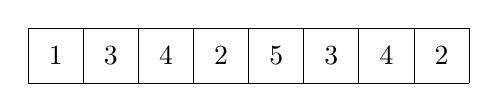
\begin{tikzpicture}[scale=0.7]
\draw (0,0) grid (8,1);

\node at (0.5,0.5) {$1$};
\node at (1.5,0.5) {$3$};
\node at (2.5,0.5) {$4$};
\node at (3.5,0.5) {$2$};
\node at (4.5,0.5) {$5$};
\node at (5.5,0.5) {$3$};
\node at (6.5,0.5) {$4$};
\node at (7.5,0.5) {$2$};
\end{tikzpicture}
\end{center}

First, the elements 1, 3 and 4 are added to the stack,
because each element is larger than the previous element.
Thus, the nearest smaller element of 4 is 3,
and the nearest smaller element of 3 is 1.
\begin{center}
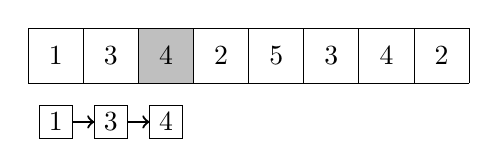
\begin{tikzpicture}[scale=0.7]
\fill[color=lightgray] (2,0) rectangle (3,1);
\draw (0,0) grid (8,1);

\node at (0.5,0.5) {$1$};
\node at (1.5,0.5) {$3$};
\node at (2.5,0.5) {$4$};
\node at (3.5,0.5) {$2$};
\node at (4.5,0.5) {$5$};
\node at (5.5,0.5) {$3$};
\node at (6.5,0.5) {$4$};
\node at (7.5,0.5) {$2$};

\draw (0.2,0.2-1.2) rectangle (0.8,0.8-1.2);
\draw (1.2,0.2-1.2) rectangle (1.8,0.8-1.2);
\draw (2.2,0.2-1.2) rectangle (2.8,0.8-1.2);

\node at (0.5,0.5-1.2) {$1$};
\node at (1.5,0.5-1.2) {$3$};
\node at (2.5,0.5-1.2) {$4$};

\draw[->,thick] (0.8,0.5-1.2) -- (1.2,0.5-1.2);
\draw[->,thick] (1.8,0.5-1.2) -- (2.2,0.5-1.2);
\end{tikzpicture}
\end{center}

The next element 2 is smaller than the two top
elements in the stack.
Thus, the elements 3 and 4 are removed from the stack,
and then the element 2 is added to the stack.
Its nearest smaller element is 1:
\begin{center}
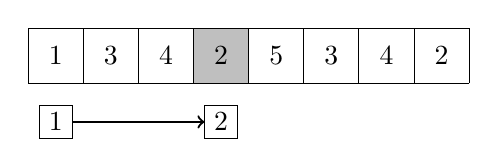
\begin{tikzpicture}[scale=0.7]
\fill[color=lightgray] (3,0) rectangle (4,1);
\draw (0,0) grid (8,1);

\node at (0.5,0.5) {$1$};
\node at (1.5,0.5) {$3$};
\node at (2.5,0.5) {$4$};
\node at (3.5,0.5) {$2$};
\node at (4.5,0.5) {$5$};
\node at (5.5,0.5) {$3$};
\node at (6.5,0.5) {$4$};
\node at (7.5,0.5) {$2$};

\draw (0.2,0.2-1.2) rectangle (0.8,0.8-1.2);
\draw (3.2,0.2-1.2) rectangle (3.8,0.8-1.2);

\node at (0.5,0.5-1.2) {$1$};
\node at (3.5,0.5-1.2) {$2$};

\draw[->,thick] (0.8,0.5-1.2) -- (3.2,0.5-1.2);
\end{tikzpicture}
\end{center}

Then, the element 5 is larger than the element 2,
so it will be added to the stack, and
its nearest smaller element is 2:
\begin{center}
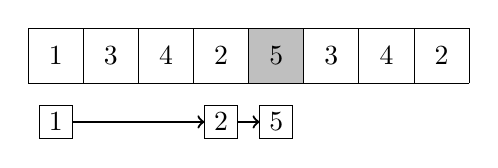
\begin{tikzpicture}[scale=0.7]
\fill[color=lightgray] (4,0) rectangle (5,1);
\draw (0,0) grid (8,1);

\node at (0.5,0.5) {$1$};
\node at (1.5,0.5) {$3$};
\node at (2.5,0.5) {$4$};
\node at (3.5,0.5) {$2$};
\node at (4.5,0.5) {$5$};
\node at (5.5,0.5) {$3$};
\node at (6.5,0.5) {$4$};
\node at (7.5,0.5) {$2$};

\draw (0.2,0.2-1.2) rectangle (0.8,0.8-1.2);
\draw (3.2,0.2-1.2) rectangle (3.8,0.8-1.2);
\draw (4.2,0.2-1.2) rectangle (4.8,0.8-1.2);

\node at (0.5,0.5-1.2) {$1$};
\node at (3.5,0.5-1.2) {$2$};
\node at (4.5,0.5-1.2) {$5$};

\draw[->,thick] (0.8,0.5-1.2) -- (3.2,0.5-1.2);
\draw[->,thick] (3.8,0.5-1.2) -- (4.2,0.5-1.2);
\end{tikzpicture}
\end{center}

After this, the element 5 is removed from the stack
and the elements 3 and 4 are added to the stack:
\begin{center}
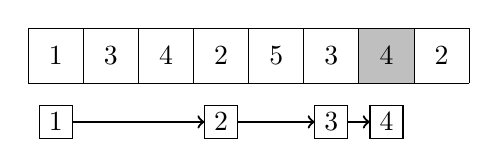
\begin{tikzpicture}[scale=0.7]
\fill[color=lightgray] (6,0) rectangle (7,1);
\draw (0,0) grid (8,1);

\node at (0.5,0.5) {$1$};
\node at (1.5,0.5) {$3$};
\node at (2.5,0.5) {$4$};
\node at (3.5,0.5) {$2$};
\node at (4.5,0.5) {$5$};
\node at (5.5,0.5) {$3$};
\node at (6.5,0.5) {$4$};
\node at (7.5,0.5) {$2$};

\draw (0.2,0.2-1.2) rectangle (0.8,0.8-1.2);
\draw (3.2,0.2-1.2) rectangle (3.8,0.8-1.2);
\draw (5.2,0.2-1.2) rectangle (5.8,0.8-1.2);
\draw (6.2,0.2-1.2) rectangle (6.8,0.8-1.2);

\node at (0.5,0.5-1.2) {$1$};
\node at (3.5,0.5-1.2) {$2$};
\node at (5.5,0.5-1.2) {$3$};
\node at (6.5,0.5-1.2) {$4$};

\draw[->,thick] (0.8,0.5-1.2) -- (3.2,0.5-1.2);
\draw[->,thick] (3.8,0.5-1.2) -- (5.2,0.5-1.2);
\draw[->,thick] (5.8,0.5-1.2) -- (6.2,0.5-1.2);
\end{tikzpicture}
\end{center}

Finally, all elements except 1 are removed
from the stack and the last element 2
is added to the stack:

\begin{center}
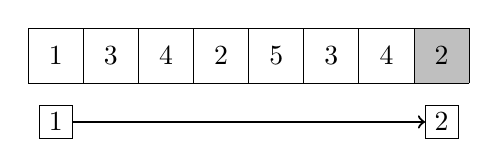
\begin{tikzpicture}[scale=0.7]
\fill[color=lightgray] (7,0) rectangle (8,1);
\draw (0,0) grid (8,1);

\node at (0.5,0.5) {$1$};
\node at (1.5,0.5) {$3$};
\node at (2.5,0.5) {$4$};
\node at (3.5,0.5) {$2$};
\node at (4.5,0.5) {$5$};
\node at (5.5,0.5) {$3$};
\node at (6.5,0.5) {$4$};
\node at (7.5,0.5) {$2$};

\draw (0.2,0.2-1.2) rectangle (0.8,0.8-1.2);
\draw (7.2,0.2-1.2) rectangle (7.8,0.8-1.2);

\node at (0.5,0.5-1.2) {$1$};
\node at (7.5,0.5-1.2) {$2$};

\draw[->,thick] (0.8,0.5-1.2) -- (7.2,0.5-1.2);
\end{tikzpicture}
\end{center}

The efficiency of the algorithm depends on
the total number of stack operations.
If the current element is larger than
the top element in the stack, it is directly
added to the stack, which is efficient.
However, sometimes the stack can contain several
larger elements and it takes time to remove them.
Still, each element is added \emph{exactly once} to the stack
and removed \emph{at most once} from the stack.
Thus, each element causes $O(1)$ stack operations,
and the algorithm works in $O(n)$ time.

\section{Sliding window minimum}

\index{sliding window}
\index{sliding window minimum}

A \key{sliding window} is a constant-size subarray
that moves from left to right through the array.
At each window position,
we want to calculate some information
about the elements inside the window.
In this section, we focus on the problem
of maintaining the \key{sliding window minimum},
which means that
we should report the smallest value inside each window.

The sliding window minimum can be calculated
using a similar idea that we used to calculate
the nearest smaller elements.
We maintain a queue
where each element is larger than
the previous element,
and the first element
always corresponds to the minimum element inside the window.
After each window move,
we remove elements from the end of the queue
until the last queue element
is smaller than the new window element,
or the queue becomes empty.
We also remove the first queue element
if it is not inside the window anymore.
Finally, we add the new window element
to the end of the queue.

As an example, consider the following array:

\begin{center}
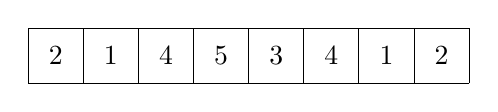
\begin{tikzpicture}[scale=0.7]
\draw (0,0) grid (8,1);

\node at (0.5,0.5) {$2$};
\node at (1.5,0.5) {$1$};
\node at (2.5,0.5) {$4$};
\node at (3.5,0.5) {$5$};
\node at (4.5,0.5) {$3$};
\node at (5.5,0.5) {$4$};
\node at (6.5,0.5) {$1$};
\node at (7.5,0.5) {$2$};
\end{tikzpicture}
\end{center}

Suppose that the size of the sliding window is 4.
At the first window position, the smallest value is 1:
\begin{center}
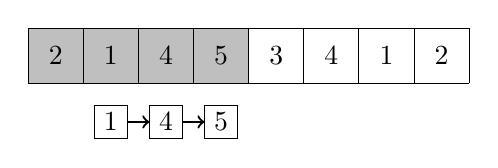
\begin{tikzpicture}[scale=0.7]
\fill[color=lightgray] (0,0) rectangle (4,1);
\draw (0,0) grid (8,1);

\node at (0.5,0.5) {$2$};
\node at (1.5,0.5) {$1$};
\node at (2.5,0.5) {$4$};
\node at (3.5,0.5) {$5$};
\node at (4.5,0.5) {$3$};
\node at (5.5,0.5) {$4$};
\node at (6.5,0.5) {$1$};
\node at (7.5,0.5) {$2$};

\draw (1.2,0.2-1.2) rectangle (1.8,0.8-1.2);
\draw (2.2,0.2-1.2) rectangle (2.8,0.8-1.2);
\draw (3.2,0.2-1.2) rectangle (3.8,0.8-1.2);

\node at (1.5,0.5-1.2) {$1$};
\node at (2.5,0.5-1.2) {$4$};
\node at (3.5,0.5-1.2) {$5$};

\draw[->,thick] (1.8,0.5-1.2) -- (2.2,0.5-1.2);
\draw[->,thick] (2.8,0.5-1.2) -- (3.2,0.5-1.2);
\end{tikzpicture}
\end{center}

Then the window moves one step right.
The new element 3 is smaller than the elements
4 and 5 in the queue, so the elements 4 and 5
are removed from the queue
and the element 3 is added to the queue.
The smallest value is still 1.
\begin{center}
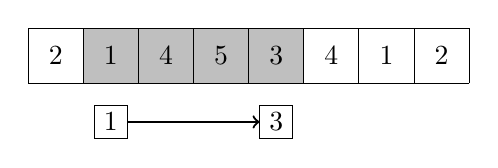
\begin{tikzpicture}[scale=0.7]
\fill[color=lightgray] (1,0) rectangle (5,1);
\draw (0,0) grid (8,1);

\node at (0.5,0.5) {$2$};
\node at (1.5,0.5) {$1$};
\node at (2.5,0.5) {$4$};
\node at (3.5,0.5) {$5$};
\node at (4.5,0.5) {$3$};
\node at (5.5,0.5) {$4$};
\node at (6.5,0.5) {$1$};
\node at (7.5,0.5) {$2$};

\draw (1.2,0.2-1.2) rectangle (1.8,0.8-1.2);
\draw (4.2,0.2-1.2) rectangle (4.8,0.8-1.2);

\node at (1.5,0.5-1.2) {$1$};
\node at (4.5,0.5-1.2) {$3$};

\draw[->,thick] (1.8,0.5-1.2) -- (4.2,0.5-1.2);
\end{tikzpicture}
\end{center}

After this, the window moves again,
and the smallest element 1
does not belong to the window anymore.
Thus, it is removed from the queue and the smallest
value is now 3. Also the new element 4
is added to the queue.
\begin{center}
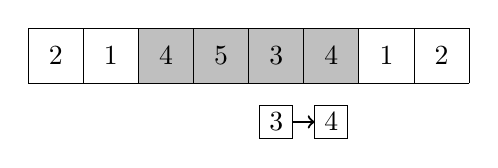
\begin{tikzpicture}[scale=0.7]
\fill[color=lightgray] (2,0) rectangle (6,1);
\draw (0,0) grid (8,1);

\node at (0.5,0.5) {$2$};
\node at (1.5,0.5) {$1$};
\node at (2.5,0.5) {$4$};
\node at (3.5,0.5) {$5$};
\node at (4.5,0.5) {$3$};
\node at (5.5,0.5) {$4$};
\node at (6.5,0.5) {$1$};
\node at (7.5,0.5) {$2$};

\draw (4.2,0.2-1.2) rectangle (4.8,0.8-1.2);
\draw (5.2,0.2-1.2) rectangle (5.8,0.8-1.2);

\node at (4.5,0.5-1.2) {$3$};
\node at (5.5,0.5-1.2) {$4$};

\draw[->,thick] (4.8,0.5-1.2) -- (5.2,0.5-1.2);
\end{tikzpicture}
\end{center}

The next new element 1 is smaller than all elements
in the queue.
Thus, all elements are removed from the queue
and it will only contain the element 1:
\begin{center}
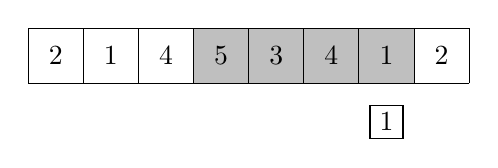
\begin{tikzpicture}[scale=0.7]
\fill[color=lightgray] (3,0) rectangle (7,1);
\draw (0,0) grid (8,1);

\node at (0.5,0.5) {$2$};
\node at (1.5,0.5) {$1$};
\node at (2.5,0.5) {$4$};
\node at (3.5,0.5) {$5$};
\node at (4.5,0.5) {$3$};
\node at (5.5,0.5) {$4$};
\node at (6.5,0.5) {$1$};
\node at (7.5,0.5) {$2$};

\draw (6.2,0.2-1.2) rectangle (6.8,0.8-1.2);

\node at (6.5,0.5-1.2) {$1$};
\end{tikzpicture}
\end{center}

Finally the window reaches its last position.
The element 2 is added to the queue,
but the smallest value inside the window
is still 1.
\begin{center}
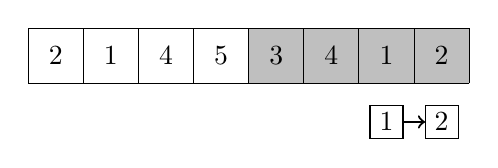
\begin{tikzpicture}[scale=0.7]
\fill[color=lightgray] (4,0) rectangle (8,1);
\draw (0,0) grid (8,1);

\node at (0.5,0.5) {$2$};
\node at (1.5,0.5) {$1$};
\node at (2.5,0.5) {$4$};
\node at (3.5,0.5) {$5$};
\node at (4.5,0.5) {$3$};
\node at (5.5,0.5) {$4$};
\node at (6.5,0.5) {$1$};
\node at (7.5,0.5) {$2$};

\draw (6.2,0.2-1.2) rectangle (6.8,0.8-1.2);
\draw (7.2,0.2-1.2) rectangle (7.8,0.8-1.2);

\node at (6.5,0.5-1.2) {$1$};
\node at (7.5,0.5-1.2) {$2$};

\draw[->,thick] (6.8,0.5-1.2) -- (7.2,0.5-1.2);
\end{tikzpicture}
\end{center}

Since each array element
is added to the queue exactly once and
removed from the queue at most once,
the algorithm works in $O(n)$ time.



